\appendix
% \crefalias{section}{app}  % treat section counter as "app" in cleveref
% \crefname{app}{Appendix}{Appendices}
% \Crefname{app}{Appendix}{Appendices}
% \setcounter{page}{1}

% \section{ The Nice property of forward process}
% \label{app:nice-property}

% This property allows us to jump directly to any noisy image $x_t$ from original image $x_0$ given a timestep $t$. Starting from the forward process equation Eq. \ref{eq:foward}: 

% $$
% q(x_t \mid x_{t-1}) = \mathcal{N}\left(x_t; \sqrt{1 - \beta_t} \, x_{t-1}, \beta_t I\right) \\ 
% $$

% Using the reparameterization trick for the Normal distribution, we can express $x_t$ as a function of a standard normal noise:

% \begin{align}
%     \epsilon \sim \mathcal{N}(0, 1) \\
%     z \sim \mathcal{N} (\mu, \sigma) \to z = \mu + \sigma . \epsilon \\
%     x_t &= \sqrt{1 - \beta_t} x_{t-1} + \sqrt{\beta_t} \epsilon \\
%     &= \sqrt{\alpha_t} x_{t-1} + \sqrt{1 - \alpha_t} \epsilon
% \end{align}

% Notice that $x_{t-1}$ can also be developed similarly, and by expanding $x_t$ recursively, we have: 

% \begin{align*}
%     x_t &= \sqrt{\alpha_t} \left( \sqrt{\alpha_{t-1}} x_{t-2} + \sqrt{1 - \alpha_{t-1}} \, \epsilon \right) + \sqrt{1 - \alpha_t} \, \epsilon \\
%     &= \sqrt{\alpha_t \alpha_{t-1}} \, x_{t-2} + \sqrt{\alpha_t (1 - \alpha_{t-1})} \, \epsilon + \sqrt{1 - \alpha_t} \, \epsilon \\
%     &= \sqrt{\alpha_t \alpha_{t-1}} \, x_{t-2} + \underbrace{\sqrt{\alpha_t (1 - \alpha_{t-1})} \, \epsilon}_{a} + \underbrace{\sqrt{1 - \alpha_t} \, \epsilon}_{b}
% \end{align*}

% The last two components in the LHS are two normal r.v, and the sum of normal random variables is a random variable, we have:

% \begin{align*}
%     a + b &\sim \mathcal{N}(0, (\alpha_t (1 - \alpha_{t-1}) + 1 - \alpha_t)\mathbf{I)} \\
%     &\sim \mathcal{N}(0, (\alpha_t - \alpha_t \alpha_{t-1} + 1 - \alpha_t) \mathbf{I})\\
%     &\sim \mathcal{N}(0, (1 - \alpha_t \alpha_{t-1})\mathbf{I}) \\
%     \to x_t &= \sqrt{\alpha_t \alpha_{t-1}} \, x_{t-2} + \sqrt{1 - \alpha_t \alpha_{t-1}} \epsilon \\
%     \text{keep on developing until $x_0$, we have:} \\
%     x_t &= \sqrt{\prod_{s=1}^{t}\alpha_s} x_0 + \sqrt{1 - \prod_{s=1}^{t}\alpha_s} \epsilon \\
%     &= \sqrt{\bar{\alpha_t}} x_0 + \sqrt{1 - \bar{\alpha_t}} \epsilon 
% \end{align*}

% Using the reparameterization trick again, we can express the conditional probability of $x_t$ given $x_0$ as: 

% \begin{align*}
%     p(x_t \mid x_0) = \mathcal{N}(x_t; \sqrt{\bar{\alpha_t}} x_0, (1 - \bar{\alpha_t})\mathbf{I})
% \end{align*}

% \chapter{Network architectures}
% \section{Spatial Diffusion Model configurations}
% \label{app:sdm-config}

% \begin{table}[h]
% \captionsetup{justification=raggedright,singlelinecheck=false}
% \caption{Spatial Diffusion Model (SDM): configurations and parameters}
% % \resizebox{\columnwidth}{!}{%

% \begin{adjustbox}{max width=0.9\textwidth}
%     \begin{tabular}{ll}
%     \toprule
%     \multicolumn{2}{l}{\textbf{Semantic Encoder $\mathrm{Enc}_{\phi}$}} \\
%     \midrule
%     Backbone & \texttt{ResNet50}\cite{ResNet50} \\
%     Pretrained Init & ImageNet \\
%     Input Modality & $1 \times 64 \times 64 $ \\
%     Output layer & \texttt{Linear(in=1000, out=512)} \\
%     Output Representation & non-spatial vector $\mathbf{y}_{sem} \in \mathbb{R}^{512}$ \\
%     \midrule
%     \multicolumn{2}{l}{\textbf{Diffusion UNet $\epsilon_{\theta}$}} \\
%     \midrule
%     Input Shape & $(B, 1, 64, 64)$, with batch size first \\
%     Channels multipliers & [32, 64, 96] \\
%     Residual Blocks per Level & 1 \\
%     Attention Resolutions (factors) & [2, 4] \\
%     Number of attention head & 1 \\
%     Conditional injection & AdaGN (scale-shift norm) \\
%     Dropout & 0.1 \\
%     Time embedded dimension & $d_{cond} = 128$ \\
%     Semantic encoder dimension & $d_{sem}=512$ \\
%     Timestep & 1000 \\
%     Beta Schedule & Linear, $\beta_t \in [10^{-4}, 2 \times 10^{-2}]$ \\
%     \midrule
%     \multicolumn{2}{l}{\textbf{Training Configuration}} \\
%     \midrule
%     Optimizer & Adam \\
%     Learning Rate & $2.5 \times 10^{-5}$ \\
%     EMA Decay & 0.999 \\
%     Train Batch Size (effective) & 20 \\
%     Training Duration & 500 epochs / $\sim$3 hours \\
%     Hardware & 2 x Nvidia L40S (45 GiB) \\
%     \bottomrule
%     \end{tabular}
% \end{adjustbox}
% % }
% \label{tab:sdm_config}
% \end{table}
% \FloatBarrier
% % \clearpage

% \section{Feature Extractor network configurations}
% \label{app:fe-config}
% \begin{table}[h]
% \captionsetup{justification=raggedright,singlelinecheck=false}
% \caption{Feature Extractor network (FE): configurations and parameters}
% % \resizebox{\columnwidth}{!}{%
% \begin{tabular}{ll}
% \toprule
% \multicolumn{2}{l}{\textbf{FE $\Phi$}} \\
% \midrule
% Backbone & \texttt{ResNet50}\cite{ResNet50} \\
% Pretrained Init & Semantic Encoder $\mathrm{Enc}_{\phi}$ \\
% Architecture & Same as $\mathrm{Enc}_{\phi}$ \\
% Input Shape & $(B, 1, 64, 64)$, with leading dimension is batch size \\
% Feature layers & [\texttt{layer1, layer2, layer3}] \\
% Feature size - \texttt{layer1} & [256, 64, 64] \\
% Feature size - \texttt{layer2} & [512, 8, 8] \\
% Feature size - \texttt{layer3} & [1024, 4, 4] \\
% DDIM samle step & 100 \\
% Noise level & [100, 250, 500, 1000] \\
% $\lambda_{DL}$ & 0.1 \\
% Optimizer & Adam \\
% Learning Rate & $1.0 \times 10^{-4}$ \\
% Train Batch Size (effective) & 20 \\
% Training Duration & 100 epochs / $\sim$4 hours \\
% Hardware & 1 x Nvidia L40S (45 GiB) \\
% \bottomrule
% \end{tabular}
% % }
% \label{tab:fe_config}
% \end{table}
% \FloatBarrier
% % \clearpage

% \section{Temporal Diffusion Model configurations}
% \label{app:tdm-config}
% \begin{table}[h]
% \captionsetup{justification=raggedright,singlelinecheck=false}
% \caption{Temporal Diffusion Model (TDM): configurations and parameters}
% % \resizebox{\columnwidth}{!}{%
% \begin{tabular}{ll}
% \toprule
% \multicolumn{2}{l}{\textbf{Encoder $\mathrm{Enc}_{\omega}$}} \\
% \midrule
% Backbone & \texttt{RRDB} \cite{zhang2018RRDB} \\
% Input Modality & $1 \times 64 \times 64 $ \\
% RRDB number of blocks & 8 \\
% RRDB number of features & 64 \\
% \midrule
% \multicolumn{2}{l}{\textbf{Diffusion UNet $\epsilon_{\theta}$}} \\
% \midrule
% Input Shape & $(B, 1, 64, 64)$, with batch size first \\
% Channels multipliers & [32, 64, 128, 256] \\
% Residual Blocks per Level & 2 \\
% Conditional injection & Summarize \\
% Dropout & 0.1 \\
% Time embedded dimension & $d_{cond} = 32$ \\
% Timestep & 1000 \\
% Beta Schedule & Linear, $\beta_t \in [10^{-4}, 2 \times 10^{-2}]$ \\
% \midrule
% \multicolumn{2}{l}{\textbf{Training Configuration}} \\
% \midrule
% Optimizer & Adam \\
% Learning Rate & $2.5 \times 10^{-4}$ \\
% EMA Decay & 0.999 \\
% Train Batch Size (effective) & 20 \\
% Training Duration & 500 epochs / $\sim$4.5 hours \\
% Hardware & 1 x Nvidia L40S (45 GiB) \\
% \bottomrule
% \end{tabular}
% % }
% \label{tab:tdm_config}
% \end{table}
% \FloatBarrier

\chapter{Effect of noise level on reconstruction errors}

\cref{fig:effect-noise-example} shows an example of effect of noise level on healthy and anomalous subjects. We observe that when increasing the noise added, the reconstruction errors increase. This can be beneficial to healthy images, but it will reduce the $l1$-errors for anomalous subjects, which reduces the discriminative power of our reconstruction-based method.

\begin{figure}[htbp]
    \centering
    \begin{subfigure}{0.75\linewidth}
        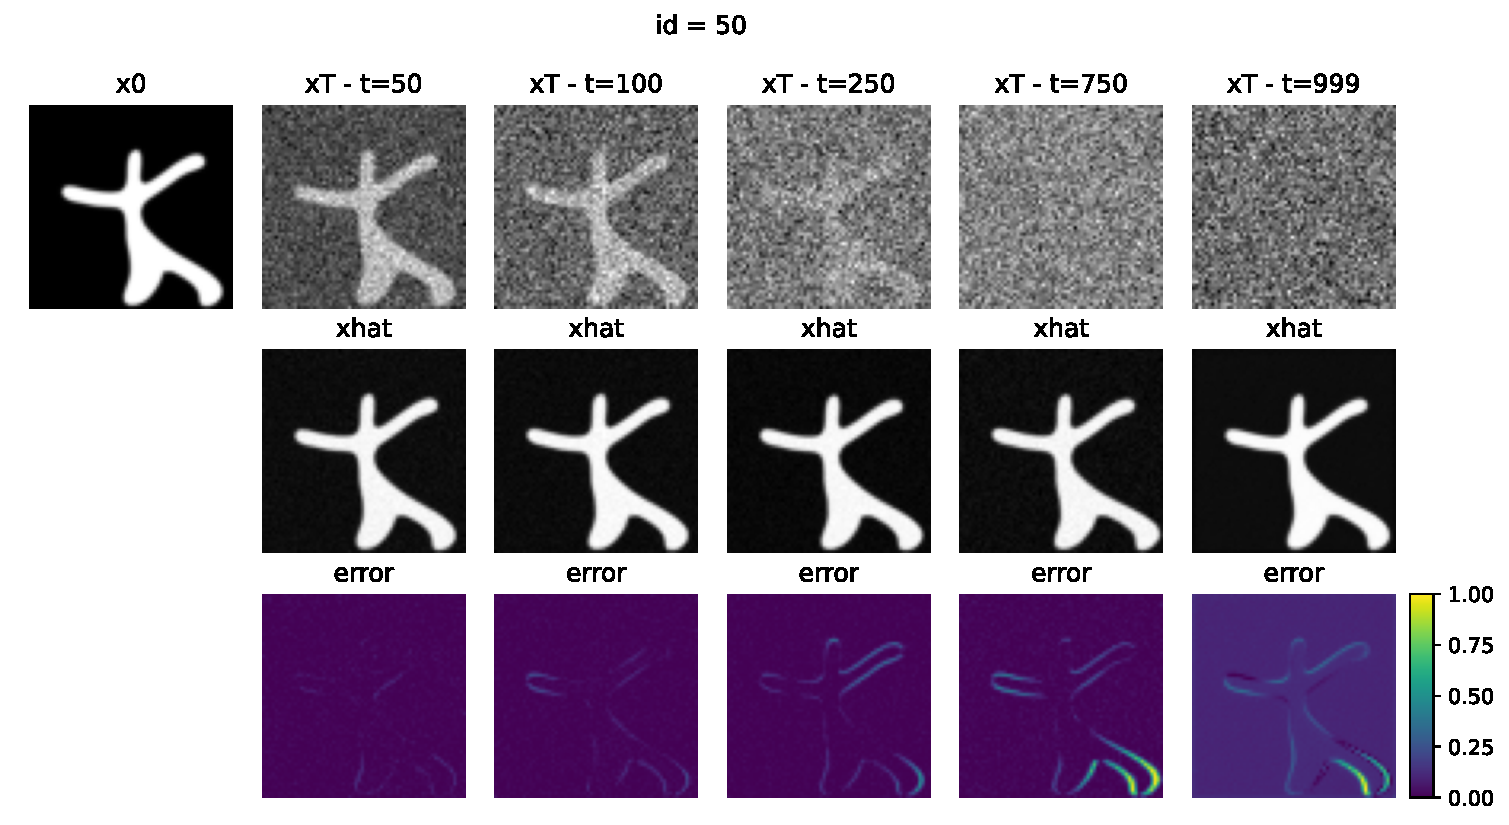
\includegraphics[width=\linewidth]{figures/effect_noise_healthy.pdf}
        \caption{Healthy subject}
    \end{subfigure}

    \begin{subfigure}{0.75\linewidth}
        \includegraphics[width=\linewidth]{figures/effect_noise_darker_circle.pdf}
        \caption{Anomaly: \texttt{darker\_circle}}
    \end{subfigure}

    \begin{subfigure}{0.75\linewidth}
        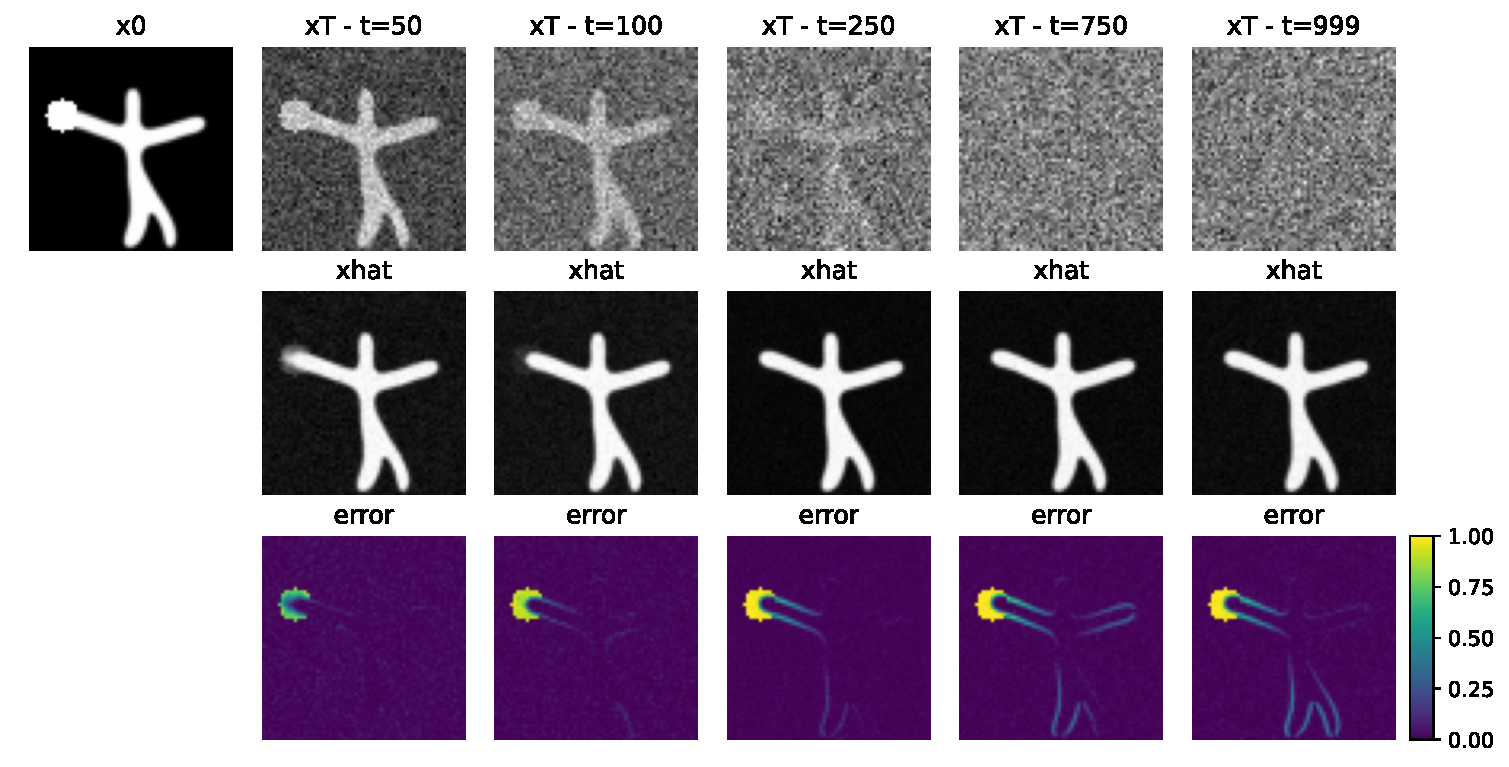
\includegraphics[width=\linewidth]{figures/effect_noise_growing_circle.pdf}
        \caption{Anomaly: \texttt{growing\_circle}}
    \end{subfigure}

    \caption{Effect of noise level on reconstructed images for healthy and anomalous subjects.}
    \label{fig:effect-noise-example}
\end{figure}

\chapter{Feature Extractor Network}
\label{app:fe-layer}

\cref{fig:fe-layers} shows an example of feature maps from our feature extractor network $\text{FE} \Phi$. Each feature map is upscaled using linear interpolation to match the original spatial resolution of original image. The color displays the highest activation values across all channels at each pixel position, which is calculated as the mean of all channels. We observe that $\Phi$ effectively captures the perceptual structure of our figures at different scales. In particular, \texttt{stage2} focuses on overall shape of the \texttt{starman}, while \texttt{stage3} highlights the importance controlled points (head, legs and hands) of each figure. \texttt{stage4} operates at smallest resolution ($4, 4$), and due to the effect of upscaling, it does not capture any meaningful part of the original images that we can exploit. This is the reason why we utilize features from \{\texttt{stage2}, \texttt{stage3}\} to calculate our feature distances. 

\begin{figure}[htbp]
    \centering
    \begin{subfigure}{0.75\linewidth} 
        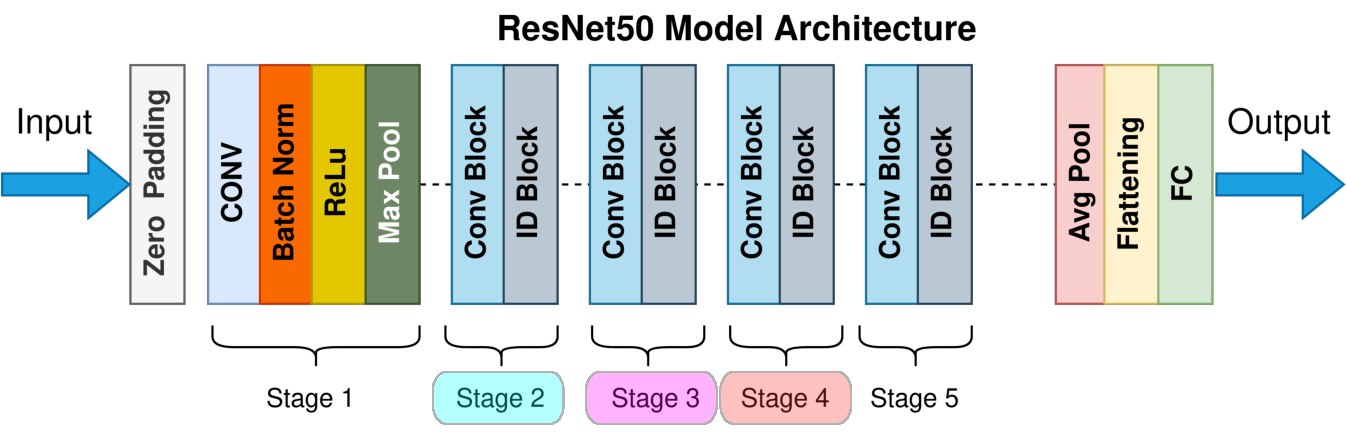
\includegraphics[width=\linewidth]{figures/resnet-50-arch.pdf}
        \caption{ResNet-50 architecture}  
        \label{fig:resnet50-arch}
    \end{subfigure}

    \begin{subfigure}{0.75\linewidth} 
        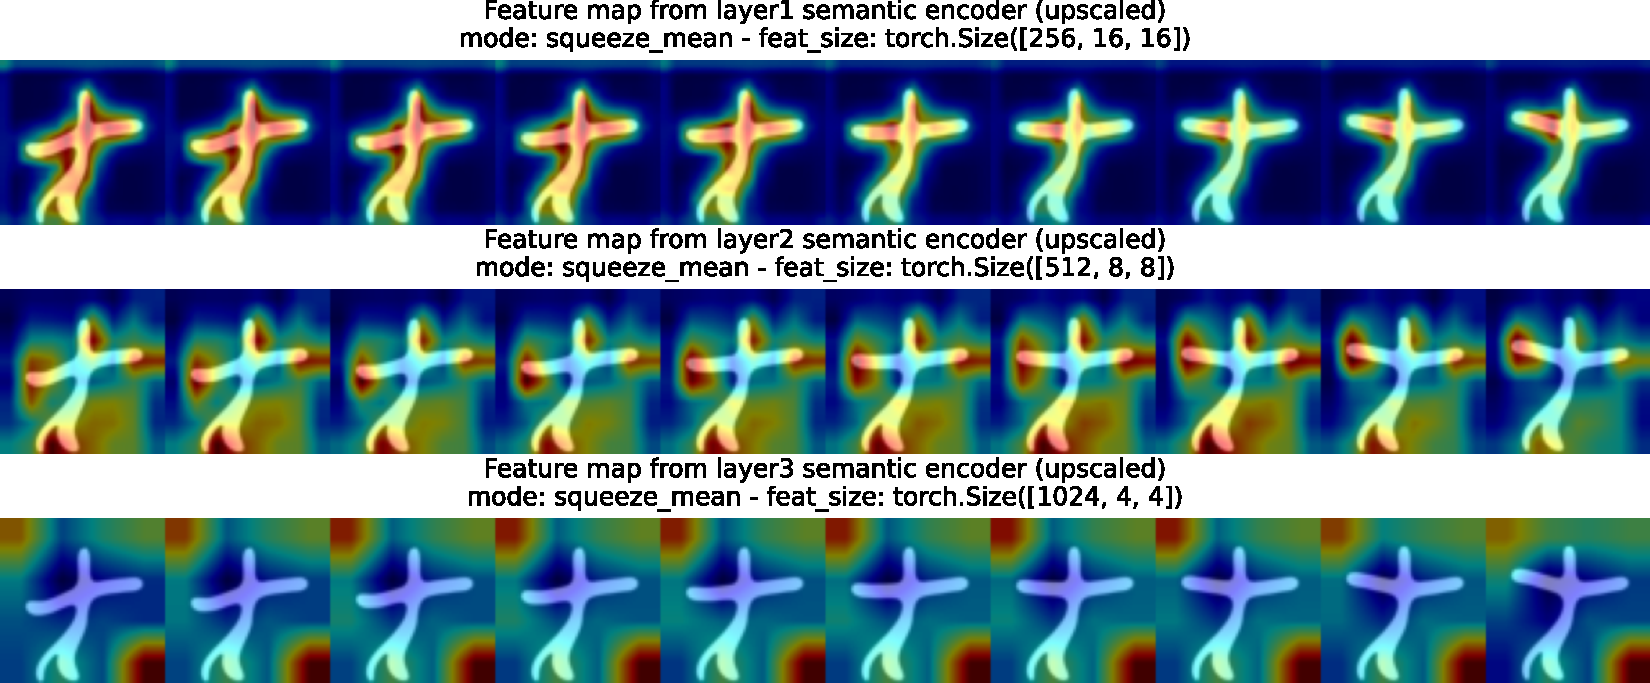
\includegraphics[width=\linewidth]{figures/fe-layer-healthy.pdf}
        \caption{Healthy subject}  
        \label{fig:fe-layer-healthy}
    \end{subfigure}

    \begin{subfigure}{0.75\linewidth} 
        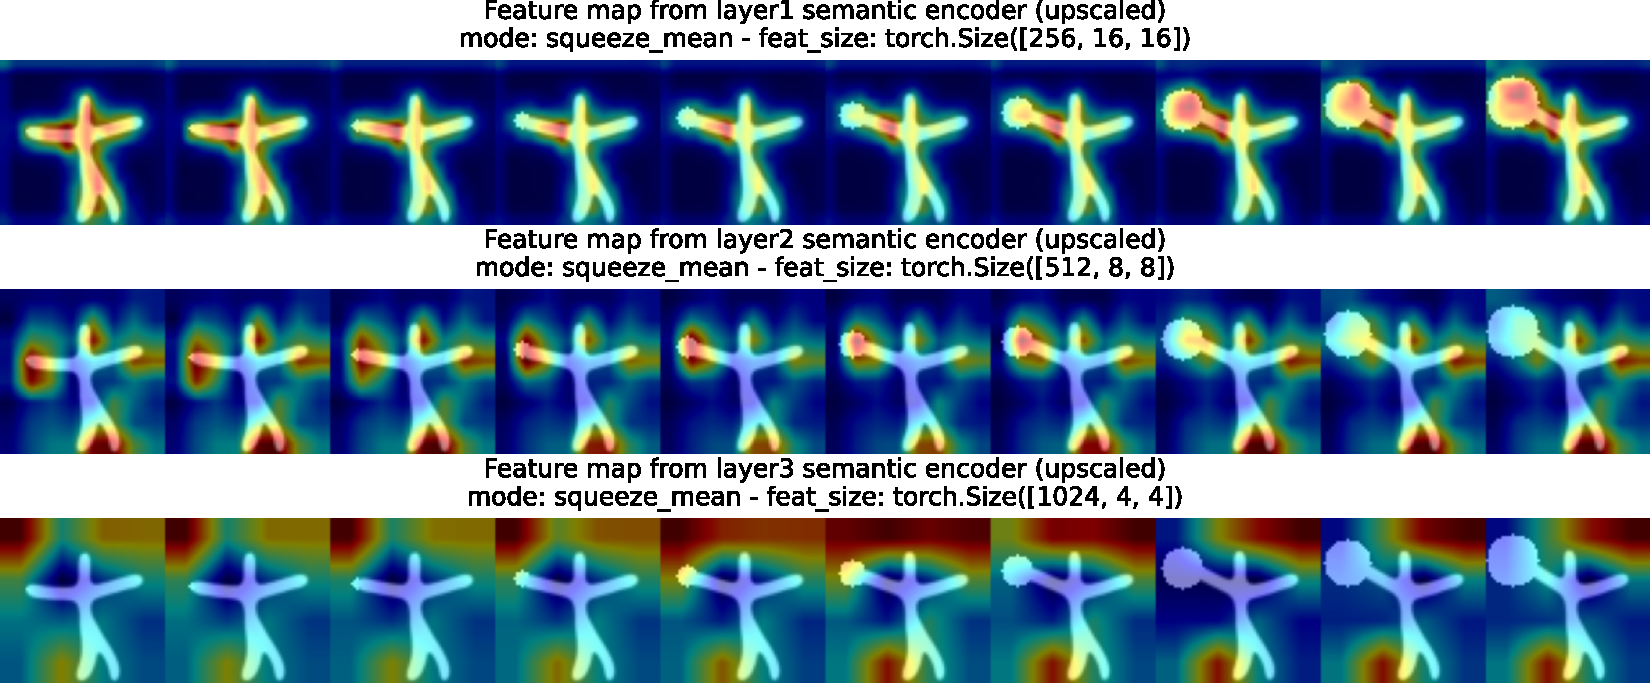
\includegraphics[width=\linewidth]{figures/fe-layer-anomaly.pdf}
        \caption{Anomaly subject}  
        \label{fig:fe-layer-anomaly}
    \end{subfigure}
    \caption[Example feature maps from semantic encoder]{Example outputs from layers of Feature Extractor network $\Phi$ in \ac{SDM}. \cref{fig:resnet50-arch} shows ResNet-50 architecture. \cref{fig:fe-layer-healthy} and \cref{fig:fe-layer-anomaly} display example of outputs for healthy and anomalous subject, respectively. Notation: \texttt{stage2}, \texttt{stage3} and \texttt{stage4} from ResNet architecture correspond to \texttt{layer1}, \texttt{layer2} and \texttt{layer3} in our paper, respectively.}
    \label{fig:fe-layers}
\end{figure}

% \clearpage
\chapter{More examples of LAFM Anomaly score maps}
\begin{figure}[htbp]
    \centering
    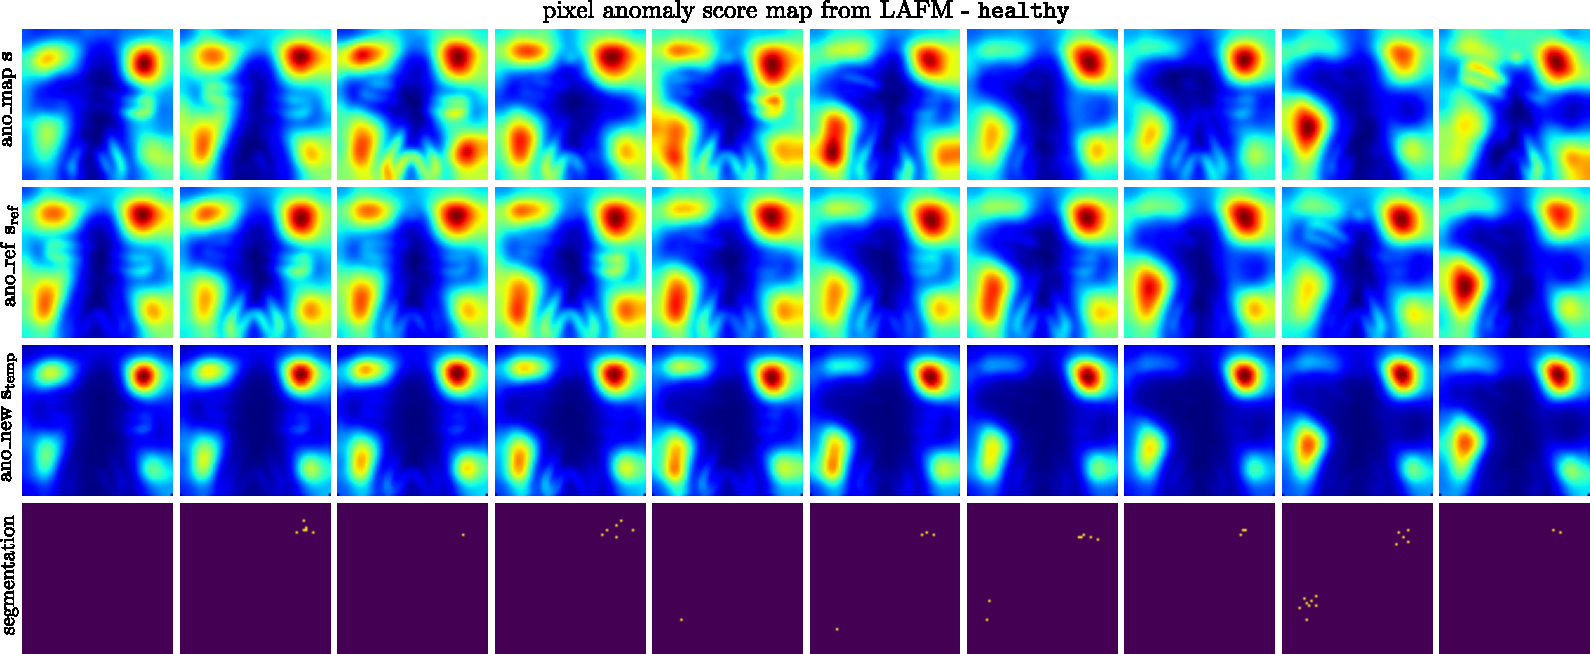
\includegraphics[width=0.75\linewidth]{figures/app-lafm-healthy.pdf}
    \caption[Example: anomaly segmentation from LAFM - \texttt{healthy} subject]{Example of anomaly score map from LAFM for healthy subject. From top to bottom: input score map (from FAM), anomaly map references, updated score map (LAFM), anomaly segmentation (Yen threshold).}   
\end{figure}

\begin{figure}[htbp]
    \centering
    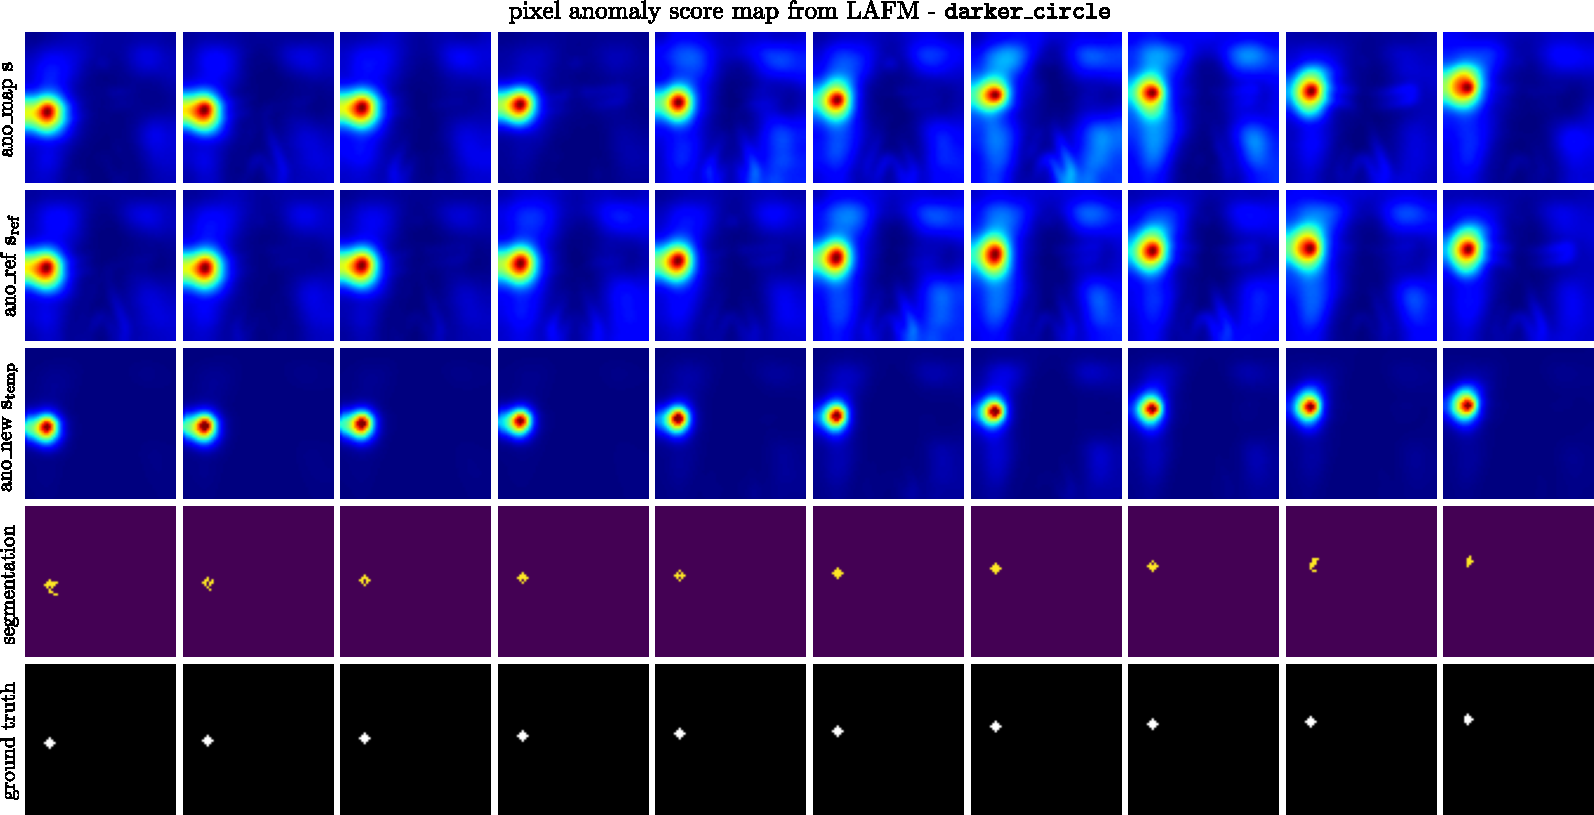
\includegraphics[width=0.75\linewidth]{figures/app-lafm-darkercircle.pdf}
    \caption[Example: anomaly segmentation from LAFM - \texttt{darker\_circle}]{Example of anomaly score map from LAFM for anomaly \texttt{darker\_circle} subject. From top to bottom: input score map (from FAM), anomaly map references, updated score map (LAFM), anomaly segmentation (Yen threshold) and ground truth annotation.}   
\end{figure}

\begin{figure}[htbp]
    \centering
    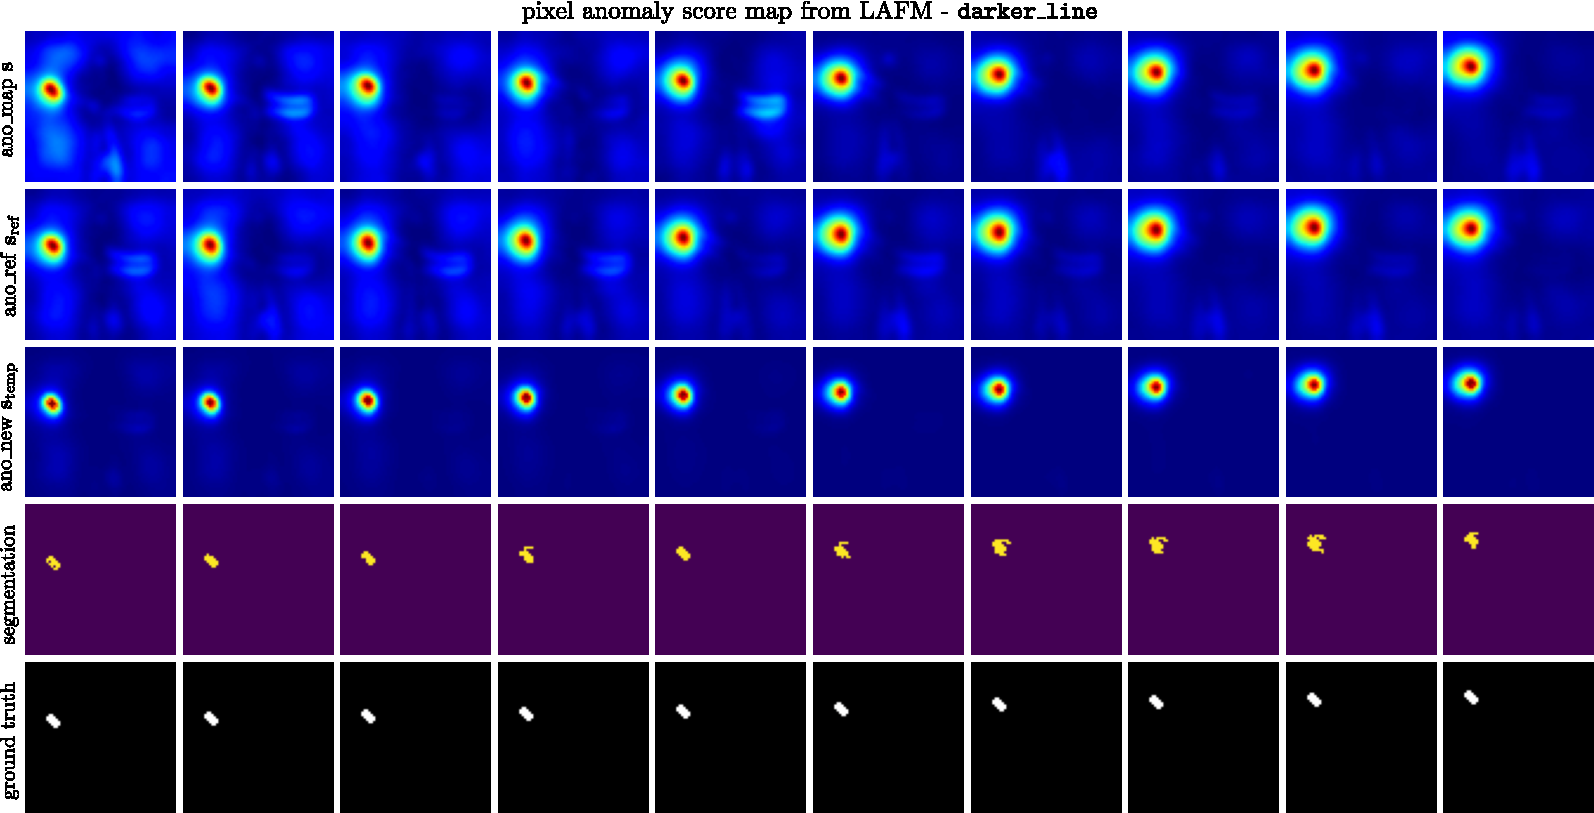
\includegraphics[width=0.75\linewidth]{figures/app-lafm-darkerline.pdf}
    \caption[Example: anomaly segmentation from LAFM - \texttt{darker\_line}]{Example of anomaly score map from LAFM for anomaly \texttt{darker\_line} subject. From top to bottom: input score map (from FAM), anomaly map references, updated score map (LAFM), anomaly segmentation (Yen threshold) and ground truth annotation.}   
\end{figure}
\FloatBarrier
